
%Dokumentinformationen	======================================================================
\newcommand{\titleinfo}{Digitaltechnik DT1 - Formelsammlung}
\newcommand{\authorinfo}{Studenten der HSR}
\newcommand{\versioninfo}{HS \ 2019}
\newcommand{\licence}{CC BY-NC-SA}


%weitere Autoren: ==========================================================================
% Dev4Future, G. Koeppel, D. Koeppel, L. Leuenberger


%eigene Befehle: ==========================================================================
%weitere neue oder umdefinierte Befehle 
\newcommand{\fb}{\color{red}\textit}	%Verweis auf Seite im Formelbuch



% Dokumenteinstellungen	 ======================================================================
%Darstellung Dokument =========================================================================================
\documentclass[10pt,twoside,a4paper,fleqn]{article}
\usepackage[left=0.5cm,right=0.5cm,top=0.5cm,bottom=0.25cm,includeheadfoot]{geometry}


%wichtige Standard-Packages ===================================================================================
\usepackage[latin1]{inputenc}
\usepackage[ngerman]{babel,varioref}
%Packages - Von LinAlg Formelsammlung kopiert! Überprüfen ob die alle notwendig sind
\usepackage{array,amsmath,amssymb,fancybox,graphicx,color,lastpage,wrapfig,fancyhdr,hyperref,verbatim,paralist}
\usepackage{listings}
%Package für Bilder im Fliesstext
\usepackage{multicol}

%Package für Tabelle im Querformat
\usepackage{rotating}


% Zusätzliche Einstellungen =============================================================================
\raggedright			% \raggedright removes paragraph indentation


%PDF Infos =============================================================================================
\hypersetup{pdfauthor={\authorinfo},pdftitle={\titleinfo},colorlinks=false}
%linkbordercolor=white
\author{\authorinfo}
\title{\titleinfo}

% Layout =================================================================================================
%Kopf- und Fusszeile
\pagestyle{fancy}
\fancyhf{}

%Linien oben und unten
\renewcommand{\headrulewidth}{0.25pt} 
\renewcommand{\footrulewidth}{0.25pt}

%Kopfzeile
\fancyhead[L]{\titleinfo{ }\tiny{\textit{(\versioninfo)}}}
\fancyhead[R]{Seite \thepage { }von \pageref{LastPage}}

%Fusszeile
\fancyfoot[L]{\footnotesize{\authorinfo}}
\fancyfoot[C]{\footnotesize{\licence \quad $\rightarrow$ \href{https://github.com/HSR-Stud}{Github: HSR-Stud}}}
\fancyfoot[R]{\footnotesize{\today}}			% standard header mit den Packages includieren



% Sections ======================================================================
%einbinden der verschieden Sections/ Seiten/ Themen
\begin{document}
	\section{Zahlendarstellungen und Codes}

\subsection{Zahlensysteme}
	\subsubsection{Zahlensysteme ohne festen Stellenwert}
		\begin{compactitem}
			\item R�misches Zahlensystem (keine Null, kein fester Stellenwert, schlechte Unterscheidung)
		\end{compactitem}
		
	\subsubsection{Zahlensysteme mit festem Stellenwert}
		\begin{multicols}{3}
			\begin{compactitem}
				\item Babylon (Basis B = 60)
				\item Maya (Basis B = 20)
			\end{compactitem}
			\columnbreak
			\begin{compactitem}
				\item Dezimal (Basis B = 10)
				\item Bin�r (Basis B = 2)
			\end{compactitem}
			\columnbreak
			\begin{compactitem}
				\item Octal (Basis B = 8)
				\item Hexadezimal (Basis B = 16)
			\end{compactitem}
		\end{multicols}
		
		\begin{minipage}{19 cm}
			Die Wertigkeit des Symbols h�ngt von seiner Position innerhalb der Symbolkette ab:\\
			\newline
			\begin{minipage}[c]{3 cm}
				$z=\sum\limits_{k=0}^{n-1}a_k*B^k$
			\end{minipage}
			\begin{minipage}[c]{6 cm}
				z: Wert der Zahl (im Dezimalsystem)\\
				a: Nennwert der Ziffer\\
				B: Basis des Zahlensystems\\
				n: Stellenanzahl\\
			\end{minipage}
			\begin{minipage}[c]{2.4 cm}
				Bsp: $4156.78=$\\
				\newline
			\end{minipage}
			\begin{minipage}[c]{6.6 cm}
				$4*10^3+1*10^2+5*10^1+6*10^0$\\
				$+7*10^{-1}+8*10^{-2}$\\
			\end{minipage}
		
			Auch gebrochene Zahlen k�nnen nach dem gleichen Muster bin�r dargestellt werden. Wichtig ist, dass das Komma immer an einer festen Stelle steht (Festkommadarstellung). Definiert ist, dass eine Bin�rzahl 8 Ziffern (n) vor dem Komma und 4 Ziffern (m) nach dem Komma besitzt. Eine gebrochene Bin�rzahl sieht dann so aus:\\
			\newline
			$z_2=a_{n-1}a_{n-2}\dots a_1a_0.a_{-1}a_{-2}\dots a_{-m+1}a_{-m}$\\
			\newline
			Der gesuchte Zahlenwert im Dezimalsystem wird dann folgendermassen berechnet:\\
			\newline
			$z_{10}=a_{n-1}*B^{n-1}+a_{n-2}*B^{n-2}+\dots +a_0*B^0+a_{-1}*B^{-1}+a_{-2}*B^{-2}+\dots +a_{-m+1}*B^{-m+1}+a_{-m}*B^{-m}$
		\end{minipage}

\subsection{Gebr�uchliche polyadische Zahlensysteme}
	\begin{tabular}{|l|l|l|l|l|}
		\hline
			System & Basis & Stellenwerte & Ziffern & Beispiel\\
		\hline
		\hline
			Bin�r & 2 & $\dots$ $2^2$ $2^1$ $2^0$ $\dots$ & 0, 1 & $110_{(2)}=6_{(10)}$\\
		\hline
			Oktal & 8 & $\dots$ $8^2$ $8^1$ $8^0$ $\dots$ & 0, 1, 2, 3, 4, 5, 6, 7 & $273_{(8)}=187_{(10)}$\\
		\hline
			Dezimal & 10 & $\dots$ $10^2$ $10^1$ $10^0$ $\dots$ & 0, 1, 2, 3, 4, 5, 6, 7, 8, 9 & $192_{(10)}=192_{(10)}$\\
		\hline
			Hexadezimal & 16 & $\dots$ $16^2$ $16^1$ $16^0$ $\dots$ & 0, 1, 2, 3, 4, 5, 6, 7, 8, 9, A, B, C, D, E, F & $2$AFF$_{(16)}=11007_{(10)}$\\
		\hline
	\end{tabular}

\subsection{Begriffe im Zusammenhang mit dem bin�ren Zahlensystem}
	\begin{compactitem}	
		\item 
			\begin{tabbing}
				xxxxxxxxxxx\=xxxxxxxxxxxxxxxxxxxxxxxxxxxxxxxxxxxxx\kill	
				Bit (b): \>
							Binary Digit: Kleinsm�gliche Speichereinheit in der Digitaltechnik. Kann zwei m�gliche Zust�nde\\
				 		\>	annehmen: 0 und 1
			\end{tabbing}
		\item 
			\begin{tabbing}
				xxxxxxxxxxx\=xxxxxxxxxxxxxxxxxxxxxxxxxxxxxxxxxxxxx\kill	
				Byte (B): \>
							Einheit von 8 Bits. Auch genannt Oktett: 1 Oktett = 1 Byte = 8 Bit. Byte ist die Standartbezeichnung\\
						\>	von Speicherkapazit�ten und Datenmengen.
			\end{tabbing}
		\item 
			\begin{tabbing}
				xxxxxxxxxxx\=xxxxxxxxxxxxxxxxxxxxxxxxxxxxxxxxxxxxx\kill	
				Nibble: \>
							Bin�rzahlen in Gruppen von 4 Bits
			\end{tabbing}
		\item 
			\begin{tabbing}
				xxxxxxxxxxx\=xxxxxxxxxxxxxxxxxxxxxxxxxxxxxxxxxxxxx\kill	
				MSB: \>
							Most Significant Bit. Bit mit h�chster Wertigkeit, steht ganz links im bin�ren Wort
			\end{tabbing}
		\item 
			\begin{tabbing}
				xxxxxxxxxxx\=xxxxxxxxxxxxxxxxxxxxxxxxxxxxxxxxxxxxx\kill	
				LSB: \>
							Least Significant Bit. Bit mit tiefster Wertigkeit, steht ganz rechts im bin�ren Wort
			\end{tabbing}
	\end{compactitem}
	
\subsection{Umwandlung von Dezimalzahlen}
	Beispiel f�r die Umwandlung der Zahl $109.78125_{(10)}$:
	\begin{tabular}{|lllllll|lllllll|lllllll|}
		\hline
			\multicolumn{7}{|l|}{Dezimal zu Bin�r} & \multicolumn{7}{|l|}{Dezimal zu Oktal} & \multicolumn{7}{|l|}{Dezimal zu Hexadeximal}\\
		\hline
		\hline
			109 & : & 2 & = & 54 & Rest: & 1 &
			109 & : & 8 & = & 13 & Rest: & 5 & 
			109 & : & 16 & = & 6 & Rest: & D \\
			
			54 & : & 2 & = & 27 & Rest: & 0 &
			13 & : & 8 & = & 1 & Rest: & 5 & 
			6 & : & 16 & = & 0 & Rest: & 6 \\
			
			27 & : & 2 & = & 13 & Rest: & 1 &
			1 & : & 8 & = & 0 & Rest: & 1 & 
			\multicolumn{7}{|l|}{} \\
						
			13 & : & 2 & = & 6 & Rest: & 1 &
			\multicolumn{7}{|l|}{} & 
			\multicolumn{7}{|l|}{} \\
			
			6 & : & 2 & = & 3 & Rest: & 0 &
			\multicolumn{7}{|l|}{} & 
			\multicolumn{7}{|l|}{} \\
			
			3 & : & 2 & = & 1 & Rest: & 1 &
			\multicolumn{7}{|l|}{} & 
			\multicolumn{7}{|l|}{} \\
			
			1 & : & 2 & = & 0 & Rest: & 1 &
			\multicolumn{7}{|l|}{} & 
			\multicolumn{7}{|l|}{} \\
		\hline
			0.78125 & * & 2 & = & 0.5625 & + & 1 &
			0.78125 & * & 8 & = & 0.25 & + & 6 &
			0.78125 & * & 16 & = & 0.5 & + & C \\
			
			0.5625 & * & 2 & = & 0.125 & + & 1 &
			0.25 & * & 8 & = & 0 & + & 2 &
			0.5 & * & 16 & = & 0 & + & 8 \\
			
			0.125 & * & 2 & = & 0.25 & + & 0 &
			\multicolumn{7}{|l|}{} &
			\multicolumn{7}{|l|}{} \\
			
			0.25 & * & 2 & = & 0.5 & + & 0 &
			\multicolumn{7}{|l|}{} &
			\multicolumn{7}{|l|}{} \\
			
			0.5 & * & 2 & = & 0 & + & 1 &
			\multicolumn{7}{|l|}{} &
			\multicolumn{7}{|l|}{} \\
		\hline
		\hline
			\multicolumn{7}{|l|}{$109_{(10)}=1101101.11001_{(2)}$} & \multicolumn{7}{|l|}{$109_{(10)}=155.62_{(8)}$} & \multicolumn{7}{|l|}{$109_{(10)}=6$D$.$C$8_{(16)}$}\\
		\hline
	\end{tabular}
	
\subsection{Addition}
	\begin{multicols}{3}
		\subsubsection{Ganzzahlen}
			\includegraphics[width=0.3\textwidth]{pics/addition1.jpg}
		\columnbreak
		
		\subsubsection{Festkommazahlen}
			\includegraphics[width=0.3\textwidth]{pics/addition2.jpg}
		\columnbreak
		
		\subsubsection{Vorzeichen-Darstellung}
			\begin{minipage}[c]{1.5 cm}
				Es gilt: 
				\newline
			\end{minipage}
			\begin{minipage}[c]{3.5 cm}
				\begin{compactitem}
					\item 0$\rightarrow$positiv
					\item 1$\rightarrow$negativ
				\end{compactitem}
			\end{minipage}
			Beispiel:\\
			\begin{tabular}{llll}
				$+$ & 12310 & = & 0 111 1011\\
				$-$ & 12310 & = & 1 111 1011\\
			\end{tabular}
	\end{multicols}

\begin{multicols}{2}
	\subsection{Einerkomplement}
		Das Einerkomplement wird durch Invertieren aller Bits der positiven Zahl gebildet.\\
		$A_{k1}=\overline{A}$\\
		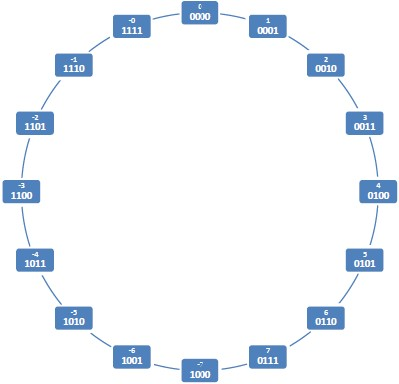
\includegraphics[width=0.4\textwidth]{pics/einerkomplement.jpg}	
		\columnbreak
		
	\subsection{Zweierkomplement}
		Das Zweierkomplement wird durch Invertieren aller Bits der positiven Zahl und der Addition von 1 gebildet.\\
		$A_{k2}=\overline{A}+1=(2^n-A)$\\
		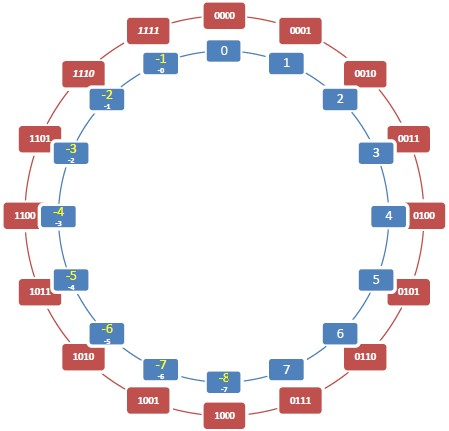
\includegraphics[width=0.4\textwidth]{pics/zweierkomplement.jpg}
\end{multicols}

\subsection{Subtraktion}
	F�r die Subtraktion A$-$B=C sind folgende Schritte notwendig:
	\begin{compactitem}
		\item 1) Der Subtrahend B muss ins Zweierkomplement gebracht werden.
		\item 2) Die arithmetische Operation muss durchgef�hrt werden.
		\item 3) Das Resultat muss korrekt interpretiert werden.
	\end{compactitem}
	In der Praxis bedeutet die Subtraktion von $2^n$, dass das Bit, welches an h�chster Stelle ($n+1$) steht, ignoriert wird.

\subsection{Bereichs�berschreitung}
	Bei Hardware ist die Wortbreite immer begrenzt, so kann es passieren, dass diese Wortbreite bei einer arithmetischen Operation �berschritten wird.\\
	Mit diesem Verfahren kann gepr�ft werden, ob eine Ergebnis korrekt ist:\\
	\ \newline
	\begin{tabular}{|l|l|l|}
		\hline
			Operation & Richtiges Ergebnis & �berlauf \\
		\hline
		\hline
			A$+$B & c$_n=0$, c$_{n-1}=0$ & c$_n=0$, c$_{n-1}=1$ \\
			A$-$B & c$_n=$c$_{n-1}$ & Nicht m�glich \\
			$-$A$-$B & c$_n=1$, c$_{n-1}=1$ & c$_n=1$, c$_{n-1}=0$ \\
		\hline		
	\end{tabular}
	
\subsection{Codes}
	\begin{minipage}[c]{5 cm}
		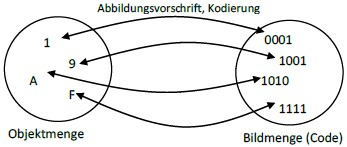
\includegraphics[width=0.9\textwidth]{pics/codes.jpg}
	\end{minipage}
	\begin{minipage}[c]{13 cm}
		Folgende Codes werden am h�ufigsten gebraucht:
		\begin{compactitem}
			\item Bin�rcode
			\item 
				\begin{tabbing}
					xxxxxxxxxxxxxxx\=xxxxxxxxxxxxxxxxxxxxxxxxxxxxxxxx\kill	
					Reiner Dualcode: \> Zuordnung von Dezimalzahlen den Bitfolgen des Dualsystems
				\end{tabbing}
			\item 
				\begin{tabbing}
					xxxxxxxxxxxxxxx\=xxxxxxxxxxxxxxxxxxxxxxxxxxxxxxxx\kill
					BCD Code: \> 
								\begin{tabular}{|lllllll|}
									\hline
										Dezimal & 1 & 2 & 3 & $\dots$ & 9 & \textgreater 9 \\
										BCD & 0001 & 0010 & 0011 & $\dots$ & 1001 & ung�ltig\\
									\hline
								\end{tabular}
				\end{tabbing}
		\end{compactitem}
	\end{minipage}
	\section{Rechenarten}
	\begin{multicols}{2}
		\subsection{Einerkomplement}
			Das Einerkomplement wird durch Invertieren aller Bits der positiven Zahl gebildet.\\
			$\mathbf{A_{k1}=\overline{A}}$\\
			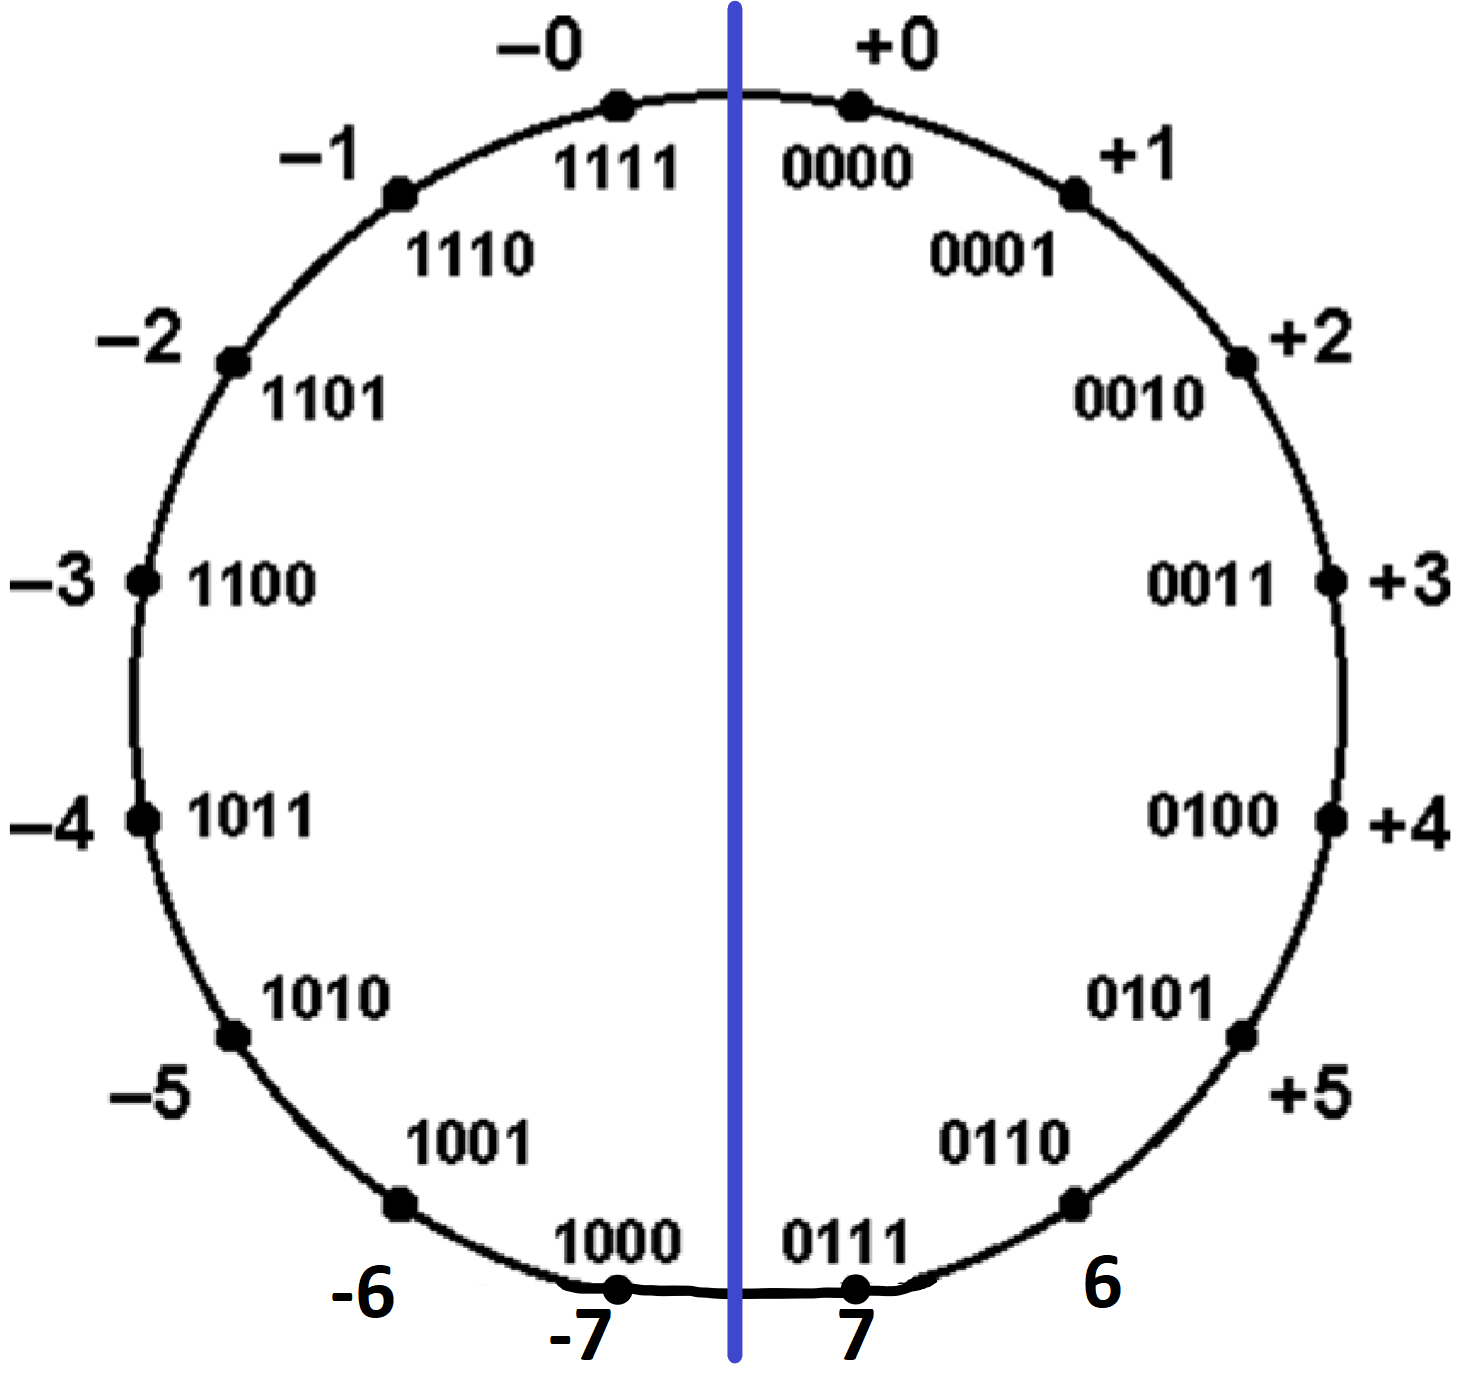
\includegraphics[width=0.4\textwidth]{pics/zahlensysteme/einerkomplement.png}	
			\columnbreak
			
		\subsection{Zweierkomplement}
			Das Zweierkomplement wird durch Invertieren aller Bits der positiven Zahl und der Addition von 1 gebildet.\\
			$\mathbf{A_{k2}=\overline{A}+1}=(2^n-A)$\\
			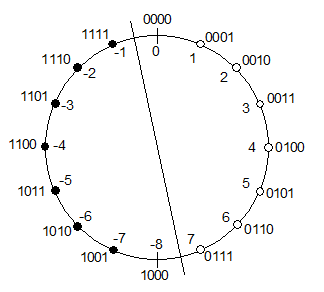
\includegraphics[width=0.4\textwidth]{pics/zahlensysteme/zweierkomplement.png}
	\end{multicols}

\subsection{Addition}
	\begin{multicols}{3}
		\subsubsection{Ganzzahlen}
		\includegraphics[width=0.3\textwidth]{pics/zahlensysteme/addition1.jpg}
		%\columnbreak
		
		\subsubsection{Festkommazahlen}
		\includegraphics[width=0.3\textwidth]{pics/zahlensysteme/addition2.jpg}
		%\columnbreak
		
		\subsubsection{Vorzeichen-Darstellung}
		\begin{minipage}[c]{1.5 cm}
			Es gilt: 
			\newline
		\end{minipage}
		\begin{minipage}[c]{3.5 cm}
			\begin{compactitem}
				\item 0$\rightarrow$positiv
				\item 1$\rightarrow$negativ
			\end{compactitem}
		\end{minipage}
		Beispiel:\\
		\begin{tabular}{llll}
			$+$ & 12310 & = & 0 111 1011\\
			$-$ & 12310 & = & 1 111 1011\\
		\end{tabular}
	\end{multicols}

\subsection{Subtraktion}
	F"ur die Subtraktion A$-$B=C sind folgende Schritte notwendig:
	\begin{compactitem}
		\item 1) Der Subtrahend B muss ins Zweierkomplement gebracht werden.
		\item 2) Die arithmetische Operation muss durchgef"uhrt werden.
		\item 3) Das Resultat muss korrekt interpretiert werden.
	\end{compactitem}
	In der Praxis bedeutet die Subtraktion von $2^n$, dass das Bit, welches an h"ochster Stelle ($n+1$) steht, ignoriert wird.
	

\subsection{Bereichs"uberschreitung}
	Bei Hardware ist die Wortbreite immer begrenzt, so kann es passieren, dass diese Wortbreite bei einer arithmetischen Operation "uberschritten wird.
	Mit diesem Verfahren kann gepr"uft werden, ob eine Ergebnis korrekt ist:\\
	\ \newline
	\begin{tabular}{|l|l|l|}
		\hline
			Operation & Richtiges Ergebnis & "Uberlauf \\
		\hline
		\hline
			A$+$B & c$_n=0$, c$_{n-1}=0$ & c$_n=0$, c$_{n-1}=1$ \\
			A$-$B & c$_n=$c$_{n-1}$ & Nicht m"oglich \\
			$-$A$-$B & c$_n=1$, c$_{n-1}=1$ & c$_n=1$, c$_{n-1}=0$ \\
		\hline		
	\end{tabular}

	\begin{multicols}{2}
		\subsubsection{Addition positiver Zahlen}
		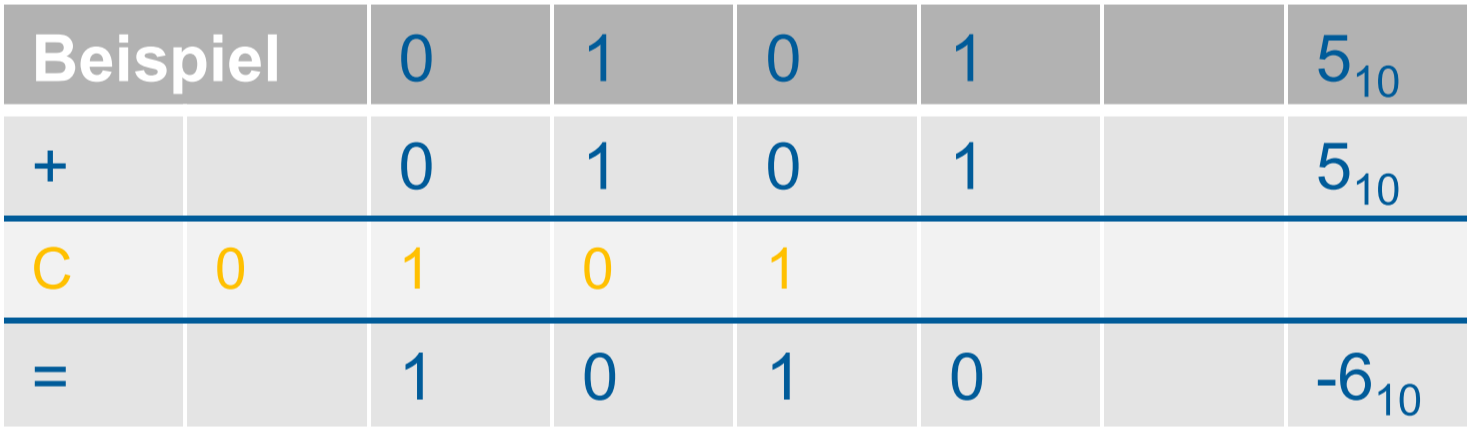
\includegraphics[width=0.45\textwidth]{pics/zahlensysteme/addition_posZahlen.png}
		%\columnbreak
		
		\subsubsection{Addition negativer Zahlen}
		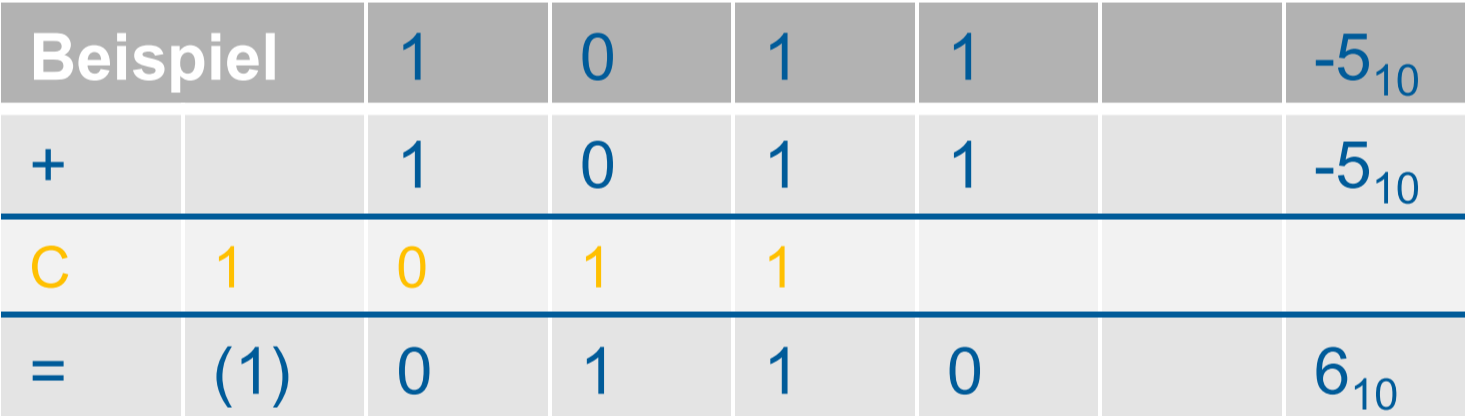
\includegraphics[width=0.45\textwidth]{pics/zahlensysteme/addition_negZahlen.png}
		%\columnbreak
	\end{multicols}
	\section{Schaltalgebra}
\subsection{Symbolik}
	Folgende Symbole werden verwendet:\\
	\begin{multicols}{4}
		$\neg=^-=$NOT
	\columnbreak
	
		$\vee=+=$OR
	\columnbreak
	
		$\wedge=*=$AND
	\columnbreak
	
		$\oplus=\$=$EXOR
	\end{multicols}
	
\subsection{Rechenregeln}
	\begin{tabular}{llll}
		Verkn"upfung mit 0 & $ a \vee 0 = a $ & $ a \wedge 0 = 0 $ & $ a \oplus 0 = a $\\
		Verkn"upfung mit 1 & $ a \vee 1 = 1 $ & $ a \wedge 1 = a $ & $ a \oplus 1 = \overline{a} $ \\
		Verkn. mit sich selbst & $ a \vee a = a $ & $ a \wedge a = a $ & $ a \oplus a = 0 $ \\
		Verkn. mit Inversem & $ a \vee \overline{a} = 1 $ & $ a \wedge \overline{a} = 0 $ & $ a \oplus \overline{a} = 1 $ \\
		\\
		Kommutativgesetz & $ a \vee b = b \vee a $ & $ a \wedge b = b \wedge a $ & $ a \oplus b = b \oplus a $\\
		Assioziativgesetz & $ (a \vee b) \vee c = a \vee (b \vee c) $ & $ (a \wedge b) \wedge c = a \wedge (b \wedge c) $ & $ (a \oplus b) \oplus c = a \oplus (b \oplus c) $ \\
		Distributivgesetz & $ a \wedge (b \vee c) = (a \wedge b) \vee (a \wedge c) $ & $ a \vee (b \wedge c) = (a \vee b) \wedge (a \vee c) $ & $ a \wedge (b \oplus c) = (a \wedge b) \oplus (a \wedge c) $ \\	
		\end{tabular}
		
\subsection{Vereinfachungen}
	\begin{multicols}{4}
		$ a \vee (a \wedge b) = a $ \\
		$ a \wedge (a \vee b) = a $ 
	\columnbreak
	
		$ (a \wedge \overline{b}) \vee b = a \vee b $ \\
		$ (a \vee \overline{b}) \wedge b = a \wedge b $ 
	\columnbreak
	
		$ (a \wedge \overline{b}) \oplus b = a \vee b $ \\
		$ (a \oplus \overline{b}) \wedge b = a \wedge b $ 
	\columnbreak
		
		$ (a \wedge b) \vee (a \wedge \overline{b}) = a $\\	
		$ (a \vee b) \wedge (a \vee \overline{b}) = a $
	\end{multicols}

\subsection{Shannon und DeMorgan}
	\begin{tabular}{lll}
		Ursprungsschaltung: & Shannon & DeMorgan\\
		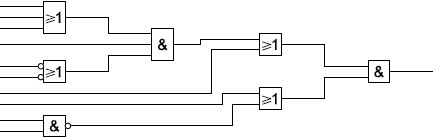
\includegraphics[width=0.3\textwidth]{pics/shanonursprung} & 
		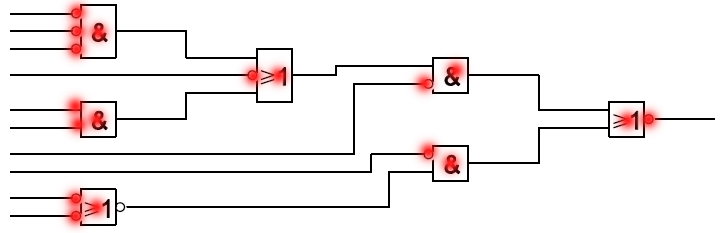
\includegraphics[width=0.3\textwidth]{pics/shanonende} &
		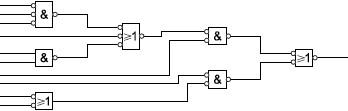
\includegraphics[width=0.3\textwidth]{pics/demorganende}\\
	\end{tabular}

\subsection{Normalformen}
	\begin{multicols}{3}
		Ausgangslage:\\
		\begin{tabular}{|l|l|l|l|l|}
			\hline	
				Dezimal & x2 & x1 & x0 & y \\	
			\hline
			\hline
				0 & 0 & 0 & 0 & 0 \\
			\hline	
				1 & 0 & 0 & 1 & 1 \\
			\hline
				2 & 0 & 1 & 0 & 0 \\
			\hline
				3 & 0 & 1 & 1 & 1 \\
			\hline
				4 & 1 & 0 & 0 & 0 \\
			\hline
				5 & 1 & 0 & 1 & d \\
			\hline
				6 & 1 & 1 & 0 & 1 \\
			\hline
				7 & 1 & 1 & 1 & 1 \\
			\hline
		\end{tabular}
		\columnbreak
		
		\subsubsection{Kanonisch disjunktive Normalform}
			\begin{tabular}{|l|}
				\hline
				\\
				\hline
					$\overline{x2} \wedge \overline{x1} \wedge x0$ \\
				\hline
				\\
				\hline
					$\overline{x2} \wedge x1 \wedge x0$ \\
				\hline
				\\
				\hline
					$[x2 \wedge \overline{x1} \wedge x0]$ \\
				\hline
					$x2 \wedge x1 \wedge \overline{x0}$ \\
				\hline
					$x2 \wedge x1 \wedge x0$ \\
				\hline	
			\end{tabular}
			$y=(\overline{x2} \wedge \overline{x1} \wedge x0) \vee (\overline{x2} \wedge x1 \wedge x0) \vee [x2 \wedge \overline{x1} \wedge x0] \vee (x2 \wedge x1 \wedge \overline{x0}) \vee (x2 \wedge x1 \wedge x0)$ \\
			Es werden nur diejenigen Zeilen der Wahrheitstabelle aufgef"uhrt, deren Funktionswert 1 oder d ist.
		\columnbreak
				
		\subsubsection{Kanonisch konjunktive Normalform}
			\begin{tabular}{|l|}
				\hline
					$x2 \vee x1 \vee x0$ \\
				\hline
				\\
				\hline
					$x2 \vee \overline{x1} \vee x0$ \\
				\hline
				\\
				\hline
					$\overline{x2} \vee x1 \vee x0$ \\
				\hline
					$[\overline{x2} \vee x1 \vee \overline{x0}]$ \\
				\hline
				\\
				\hline
				\\
				\hline	
			\end{tabular}
			$y=(x2 \vee x1 \vee x0) \wedge (x2 \vee \overline{x1} \vee x0) \wedge (\overline{x2} \vee x1 \vee x0) \wedge [\overline{x2} \vee x1 \vee \overline{x0}]$ \\
			Es werden nur diejenigen Zeilen der Wahrheitstabelle aufgef"uhrt, deren Funktionswert 0 oder d ist.
	\end{multicols}

\subsection{Karnaugh-Diagramm}
	\begin{multicols}{3}
		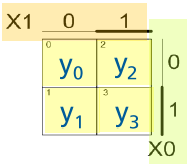
\includegraphics[width=0.3\textwidth]{pics/kv/2erKV} 
	\columnbreak
	
		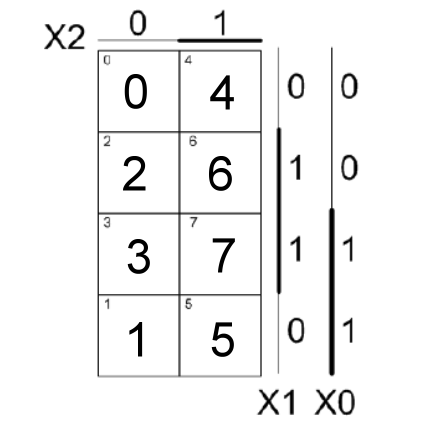
\includegraphics[width=0.3\textwidth]{pics/kv/3erKV}
	\columnbreak
	
		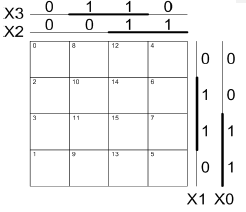
\includegraphics[width=0.3\textwidth]{pics/kv/4erKV}
	\end{multicols}
	
	\subsubsection{Arbeiten mit dem KV-Diagramm}
		\begin{compactitem}
			\item 1) \ \ Aufstellen der Wahrheitstabelle.\\
			\item 2) \ \ "Ubertragen der Werte der Wahrheitstabelle in KV Diagramm.\\
			\item 3) \ \ M"oglichst grosse Gruppen a $2^n$ Felder bilden.\\
			\item 4)
				\begin{tabular}{ll}
					Kanonisch disjunktive Normalform: & Kanonisch konjunktive Normalform: \\
					Gruppen von Feldern mit Wert 1 oder d & Gruppen von Feldern mit Wert 0 oder d\\
					Primimplikanten: AND Verkn"upfung & Primimplikanten: OR Verkn"upfung\\
					OR Verkn"upfung aller Primimplikanten & AND Verkn"upfung aller Primimplikanten\\
				\end{tabular}
		\end{compactitem}
	\section{Logische Gatter}

	\subsection{Verhalten logischer Gatter}
		\begin{multicols}{2}
			\subsubsection{St"orabstand}
				High-Pegel: $ U_{n_H} = U_{a_Hmin} - U_{e_Hmin} $\\
				Low-Pegel: $ U_{n_L} = U_{e_Lmax} - U_{a_Lmax} $\\
				
		%\end{multicols}

		%\begin{multicols}{2}
			\subsubsection{Propagation delay (Verz"ogerungszeit) }
				Zeit zwischen 50\% von $V_{max}$ am Eingang und 50\% von $V_{max}$ am Ausgang.\\
				$t_{pd}=\frac{t_{p_{LH}}+t_{p_{HL}}}{2}$\\
				
			\subsubsection{Transition time (Übergangszeit)}
				Zeit zwischen 10\% und 90\% von $V_{max}$.\\
				$t_{t_{LH}}$: Transition time low to high.\\
				$t_{t_{HL}}$: Transition time high to low.\\
				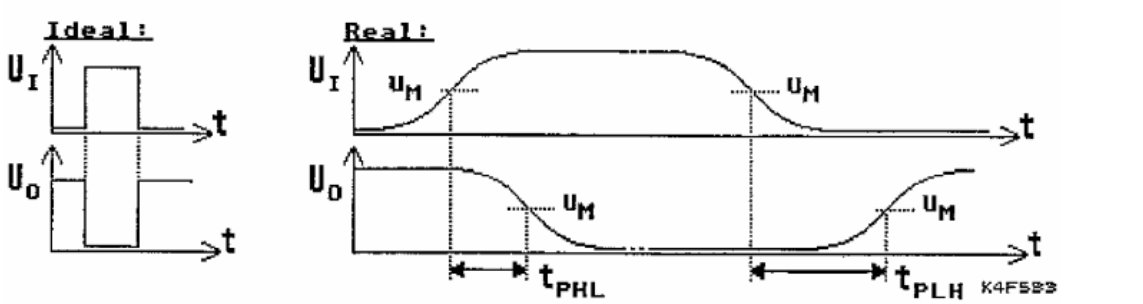
\includegraphics[width=0.2\textwidth]{pics/delay}
				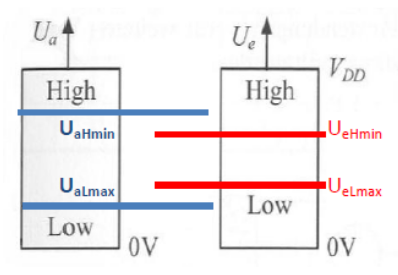
\includegraphics[width=0.2\textwidth]{pics/Pegelbereiche_Stoerabstand}
		\end{multicols}

\subsection{Hazards}
\begin{tabular}{rp{5cm}p{1cm}rp{5cm}}
	\textbf{statisch:}&kurzzeitige Änderung, obwohl keine Änderung gegeben ist.&&
	\textbf{dynamisch:}&mehrere Änderungen, obwohl nur eine Änderung gegeben ist.\\
\end{tabular}\\
\textbf{Vermeiden von Hazards:} Redundante Schaltungselemente einfügen (Fielen bei KV-Diagramm weg)
		


%\newpage
\begin{sidewaystable}
\subsection{Aufbau logischer Gatter}
\begin{tabular}{|c|c|c|c|c|c|c|c|c|}
\hline
Funktion & Buffer & NOT & AND & NAND & OR & NOR & EXOR & XNOR\\
& & Nicht & Und & Nicht Und & Oder & Nicht Oder & Exklusiv Oder & Nicht Ex. Oder\\
& & Inverter & Konjunktion & & Disjunktion & & Antivalenz & "Aquivalenz \\
\hline
Formel & a & $ \overline a $ & $ a \cdot b $ & $ \overline{a \cdot b} $ & $ a + b $ & $ \overline{a + b} $ & $ a \oplus b $ & $ \overline{a \oplus b} $\\
& a & $ \overline a $ & $ a \wedge b $ & $ \overline{a \wedge b} $ & $ a \vee b $ & $ \overline{a \vee b} $ & $ a \not= b $ & $ \overline{a \not= b} $ \\
& a & !a & $ a \& b $ & $ !(a \& b) $ & a\#b & !(a\#b) & a\$b & !(a\$b) \\
\hline
& & & & & & & &\\
& 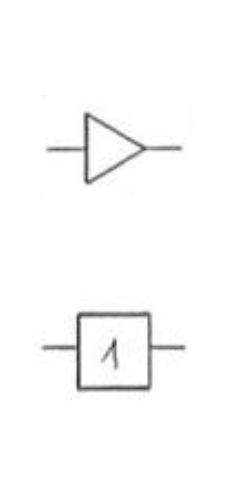
\includegraphics[width=0.08\textwidth]{pics/gates_symbol/buffer} & 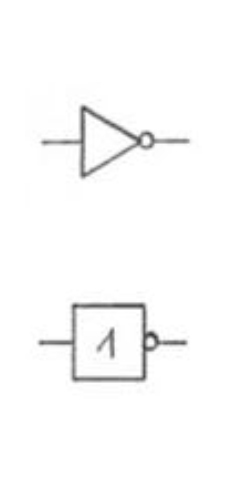
\includegraphics[width=0.08\textwidth]{pics/gates_symbol/not} & 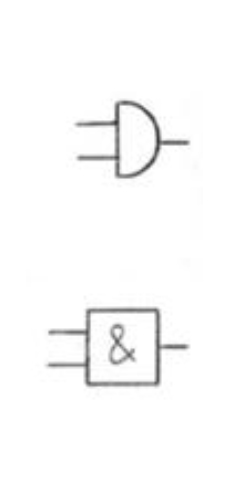
\includegraphics[width=0.08\textwidth]{pics/gates_symbol/and} & 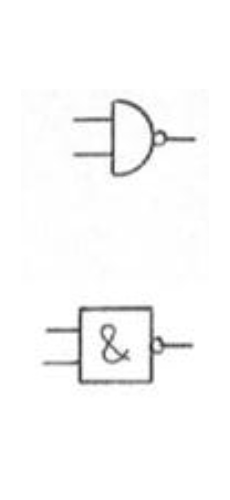
\includegraphics[width=0.08\textwidth]{pics/gates_symbol/nand} & 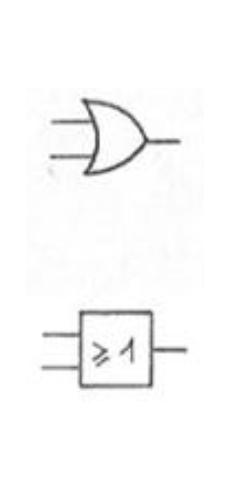
\includegraphics[width=0.08\textwidth]{pics/gates_symbol/or} & 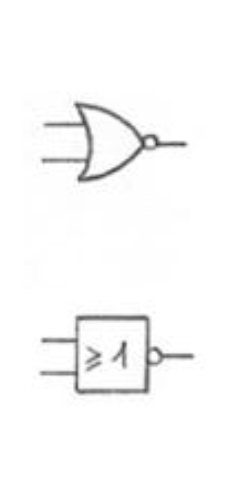
\includegraphics[width=0.08\textwidth]{pics/gates_symbol/nor} & 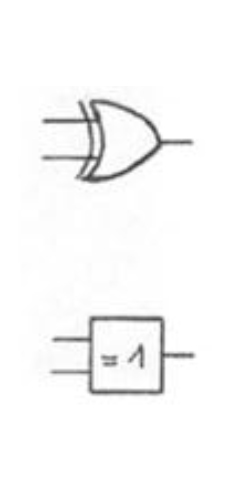
\includegraphics[width=0.08\textwidth]{pics/gates_symbol/exor} & 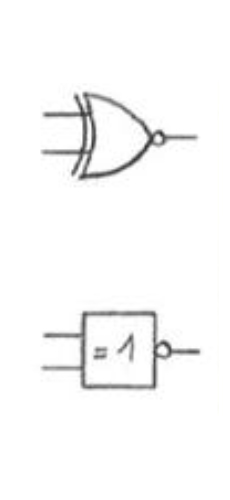
\includegraphics[width=0.08\textwidth]{pics/gates_symbol/xnor} \\
\hline
(0,0) & 0 & 1 & 0 & 1 & 0 & 1 & 0 & 1\\
(0,1) &   &   & 0 & 1 & 1 & 0 & 1 & 0\\
(1,0) & 1 & 0 & 0 & 1 & 1 & 0 & 1 & 0\\
(1,1) &   &   & 1 & 0 & 1 & 0 & 0 & 1\\
\hline
KDNF & \#(1) & \#(0) & \#(3) & \#(0,1,2) & \#(1,2,3) & \#(0) & \#(1,2) & \#(0,3) \\
KKNF & \&(0) & \&(1) & \&(0,1,2) & \&(3) & \&(0) & \&(1,2,3) & \&(0,3) & \&(1,2)\\
\hline
& & & & & & & &\\
& & 
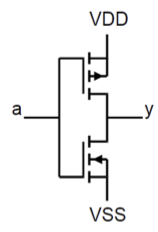
\includegraphics[width=0.12\textwidth]{pics/gates_schematic/inverter} & 
$ \overline{NAND} $ &
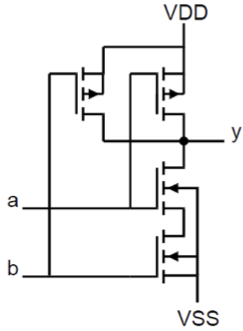
\includegraphics[width=0.12\textwidth]{pics/gates_schematic/NAND} &
$ \overline{NOR} $ &
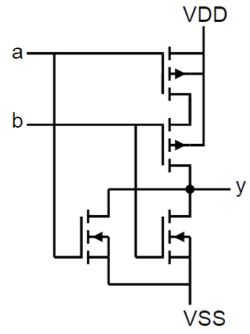
\includegraphics[width=0.12\textwidth]{pics/gates_schematic/NOR} & 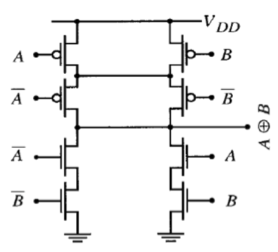
\includegraphics[width=0.12\textwidth]{pics/gates_schematic/XOR} & 
\\
\hline
\#Trans & & 2 & 6 & 4 & 6 & 4 & 8 & \\
\hline
\end{tabular}
\end{sidewaystable}
	\section{Sequentielle Systeme}

\subsection{Taktsignal}
	\begin{minipage}{8 cm}
		Weil sequentielle Schaltungen in der Regel synchron arbeiten, muss eine Referenz zur Einhaltung der Synchronit"at definiert werden. Das Taktsignal ist ein bin"are Signal, das in regelm"assiger Abfolge zwischen zwei Zust"anden hin und her pendelt.
	\end{minipage}
	\begin{minipage}{0.5 cm}
		\ 
	\end{minipage}
	\begin{minipage}{7 cm}
		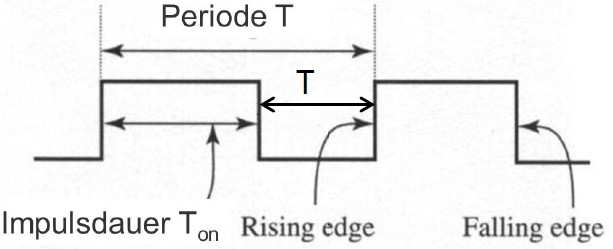
\includegraphics[width=0.9\textwidth]{pics/taktsignal}
	\end{minipage}
	\begin{minipage}{2 cm}
		$f=\frac{1}{T}$ [Hz]
	\end{minipage}

\subsection{Flipflops und Latches}
	\subsubsection{Unterschied Flipflop und Latch}
		\begin{minipage}{12 cm}
			Taktzustandsgesteuerte Systeme haben den Nachteil, dass in ihrer transparenten Phase auch asynchrone Schaltvorg"ange stattfinden k"onnen. Echt synchrone Systeme "andern ihren Zustand nur bei der aktiven Flanke des Taktsignals. Genau in diesem Moment und sonst nie wird das Eingangssignal bei einem Speicherelement in den Speicher "ubertragen. Nur beim taktflankengesteuerten System wechseln die Ausg"ange immer genau zum Zeitpunkt der aktiven Taktflanke. Beim taktzustandsgesteuerten System sind w"ahrend der transparenten Phase auch Zustands"anderungen zwischen zwei Taktflanken m"oglich. \\
			Taktflankengesteuerte Speicherelemente werden Flip-Flops genannt. Taktzustandsgesteuerte Speicherelemente werden Latches genannt
		\end{minipage}
		\begin{minipage}{0.5 cm}
			\ 
		\end{minipage}
		\begin{minipage}{6 cm}
			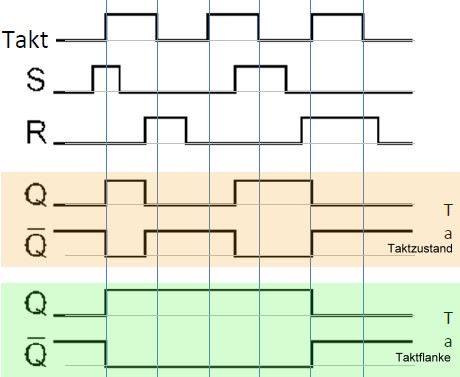
\includegraphics[width=0.9\textwidth]{pics/flipflop_latch}
		\end{minipage}
		
	\subsubsection{Transmission Gate}
		\begin{minipage}{10 cm}
			Das Transmission Gate ist von seiner Funktion her ein einfacher Schalter, der Signale sowohl auf positivem, als auch auf negativem Pegel schalten kann.
		\end{minipage}
		\begin{minipage}{0.5 cm}
			\ 
		\end{minipage}
		\begin{minipage}{8 cm}
			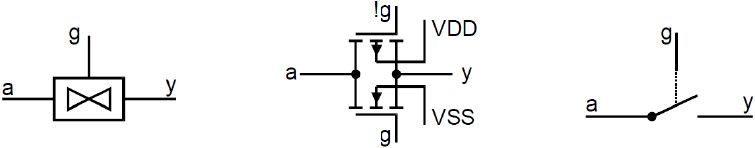
\includegraphics[width=0.9\textwidth]{pics/transmissiongate}
		\end{minipage}
		
	\begin{multicols}{2}
		\subsubsection{RS-Latch}
			\begin{minipage}{4 cm}
				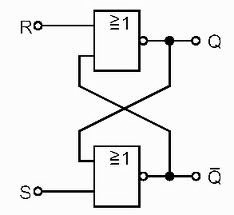
\includegraphics[width=0.9\textwidth]{pics/rs_latch}
			\end{minipage}
			\begin{minipage}{4 cm}
				\begin{tabular}{|cc|cc|}
					\hline
						S & R & $Q$ & $\overline{Q}$ \\
					\hline	
						0 & 0 & $Q$ & $\overline{Q}$ \\
						0 & 1 & 0 & 1 \\
						1 & 0 & 1 & 0 \\
						1 & 1 & \multicolumn{2}{c|}{ung"ultig} \\
					\hline
				\end{tabular}
			\end{minipage}
		
		\subsubsection{RS-Latch mit Clock}
			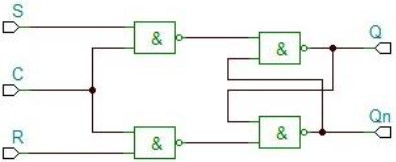
\includegraphics[width=0.4\textwidth]{pics/rs_latch_clock}
		\columnbreak
		
		\subsubsection{D-Latch}
			\begin{minipage}{4 cm}
				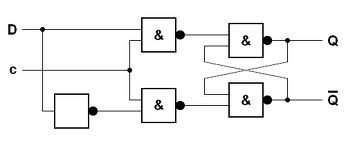
\includegraphics[width=0.9\textwidth]{pics/dlatch}
			\end{minipage}
			\begin{minipage}{4 cm}
				\begin{tabular}{|cc|cc|}
					\hline
						D & C & $Q$ & $\overline{Q}$ \\
					\hline	
						0 & 0 & $Q$ & $\overline{Q}$ \\
						0 & 1 & 0 & 1 \\
						1 & 0 & $Q$ & $\overline{Q}$ \\
						1 & 1 & 0 & 1 \\
					\hline
				\end{tabular}
			\end{minipage}
			
		\subsubsection{D-Flipflop mit Reset}
			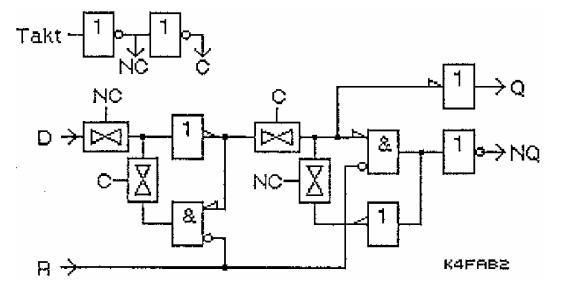
\includegraphics[width=0.4\textwidth]{pics/dflipflop}
	\end{multicols}
	
	\subsubsection{Setup- und Holdtime}
		\begin{minipage}{10 cm}
			\begin{compactitem}
				\item $t_s$= setup time $\rightarrow$ Minimale Zeitspanne, w"ahrend der ein Datensignal vor einer aktiven Clockflanke stabil sein muss, um zuverl"assig eingelesen zu werden.
				\item $t_H$= hold time $\rightarrow$ Minimale Zeitspanne, w"ahrend der ein Datensignal nach einer aktiven Clockflanke noch stabil bleiben muss, damit der Einlesevorgang des Datensignals erfolgreich abgeschlossen werden kann.
			\end{compactitem}
		\end{minipage}
		\begin{minipage}{0.5 cm}
			\ 
		\end{minipage}
		\begin{minipage}{8 cm}
			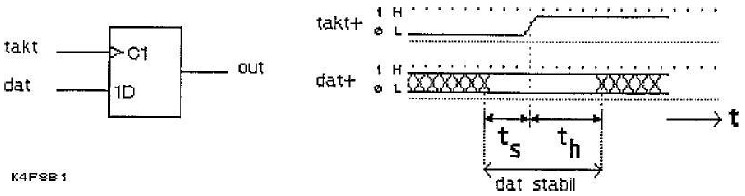
\includegraphics[width=0.9\textwidth]{pics/setupholdtime}
		\end{minipage}
		
\subsection{Beschreibung sequentieller Systeme}
	\begin{multicols}{2}
		\begin{compactitem}
			\item S: Menge der Zust"ande mit Zustandsaktionen
			\item I$\subseteq$S: Initalzust"ande
			\item T: Kombinatorische "Ubergangsrelation
			\item E: Eingangssignale
			\item A: Ausgangssignale
		\end{compactitem}
	\end{multicols}
	
	\begin{multicols}{2}
		\subsubsection{Tabellarische Beschreibung}
			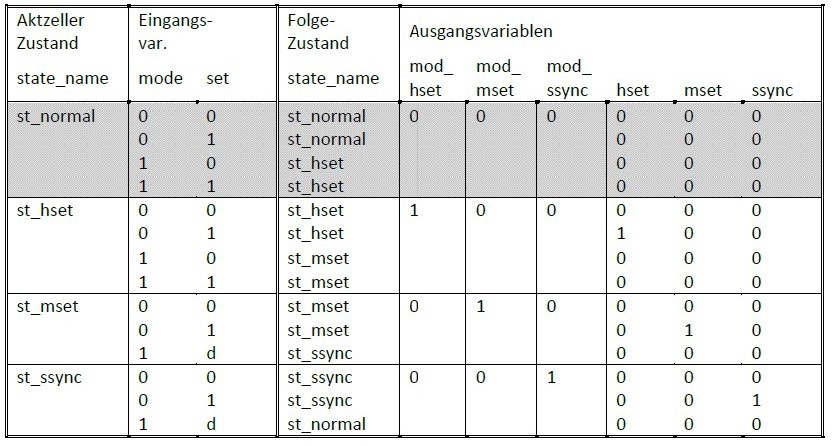
\includegraphics[width=0.49\textwidth]{pics/zustandstabelle}
		\columnbreak
		
		\subsubsection{Grafische Beschreibung (Zustandsdiagramm)}
			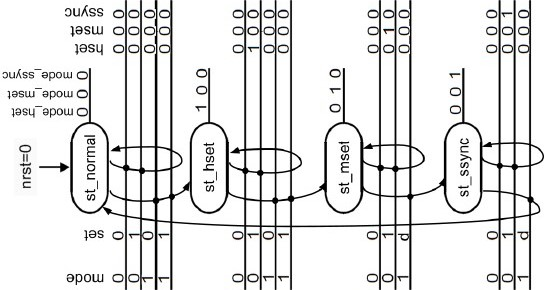
\includegraphics[width=0.5\textwidth]{pics/zustandsdiagramm}
	\end{multicols}
	Diese Beispiele visualisieren das sequentielle System des Watch-Controllers.
	
\subsection{Strukturen der Finite State Machine}
	\begin{multicols}{3}
		\subsubsection{Grundstruktur}
			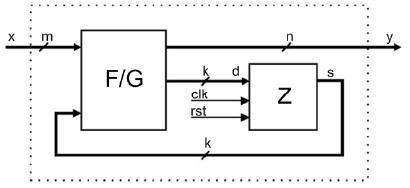
\includegraphics[width=0.3\textwidth]{pics/seq_grundstruktur}
		\columnbreak
		
			\begin{compactitem}
				\item s: Zustand, Zustandsvektor
				\item x: Prim"are Eing"ange, Eingangsvektor
				\item y: Prim"are Ausg"ange, Ausgangsvektor
				\item d: Speicheransteuerung, Folgezustand
				\item m: Anzahl Eing"ange
				\item n: Anzahl Ausg"ange
				\item k: Anzahl Speicherstellen
				\item F: Funktion f"ur die Ausg"ange
				\item G: Funktion f"ur die Speicheransteuerung
				\item Z: Zustandsspeicher
				\item I: Index der aktuellen Taktflanke (Taktflankennummer)
			\end{compactitem}
	\end{multicols}
	
	\begin{multicols}{3}
		\subsubsection{Mealy-System}
			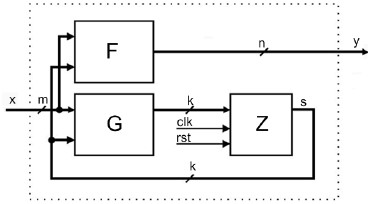
\includegraphics[width=0.26\textwidth]{pics/seq_mealy}
			Ausg"ange h"angen vom momentanen Zustand und den aktuellen Eing"angen ab
			
		\subsubsection{Moore-System}
			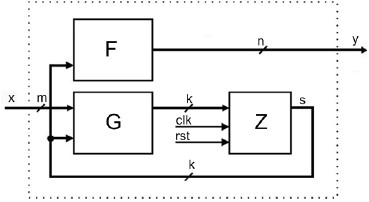
\includegraphics[width=0.26\textwidth]{pics/seq_moore}
			Ausg"ange h"angen nur vom momentanen Zustand ab und "andern mit der Clock Flanke
			
		\subsubsection{Medwedjew-System}
			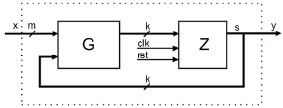
\includegraphics[width=0.3\textwidth]{pics/seq_medmedjew}
			Die prim"aren Ausg"ange entsprechen dem Zustandsvektor
	\end{multicols}
	
\subsection{Zustandscodierung}
	\begin{multicols}{3}
		\begin{compactitem}
			\item Bin"ar: Alle Zust"ande werden der Reihe nach durchnummeriert.
			\newline
			\newline
			\item ONE-HOT: Nur eine Speicherstelle im Code hat jeweils den Wert 1. Alle anderen besitzen den Wert 0 (z.B. 001, 010, 100)
			\item ONE-COLD: Nur eine Speicherstelle im Code hat jeweils den Wert 0. Alle anderen besitzen den Wert 1 (z.B. 110, 101, 011)
		\end{compactitem}
	\end{multicols}
	
\subsection{Synthese von Zustandsmaschinen}
	\begin{multicols}{2}
		\begin{enumerate}
			\setlength{\itemsep}{1pt}
			\setlength{\parskip}{0pt}
			\setlength{\parsep}{0pt}
			\item Zustandsdiagramm aufstellen
			\item Zustandskodierung zuweisen
			\item Zustandstabelle nach festen Regeln aufstellen
			\item Speicheransteuer-Funktionen bestimmen
			\item Ausgangs-Funktionen bestimmen
		\end{enumerate}
	\end{multicols}
	\begin{multicols}{2}
\section{Digital vs. Analog}
Digital ist st"orsicher, hat keine St"orfortpflanzung und erlaubt einfachen Entwurf und Test mit Hilfe von CAD.

Analog ist st"oranf"allig, komplex, erfordert Spezialisten, Entwurf weitgehend von Hand, etc.

Digital ist aber langsamer, da alles in der Welt analog ist. F"ur Digital brauchts also noch eine Umwandlung.
\subsection{AD-Wandlung}
$$ \text{Abstastfrequenz} \geq 2\cdot f_{max}$$\\
$$ \Delta \text{Quantisierungsstufe} = 2 \cdot \text{Quantisierungsfehler}$$\\
$$\text{Amplitudenauflösung: Dynamik; SNR} \approx 6dB/bit$$
\end{multicols}

\begin{multicols}{2}
\section{Digital}
\subsection{FETs (selbstsperrend)}
	\begin{tabular}{|l|c|p{2.2cm}|p{2cm}|}
		\hline
		 & & $U_{GS}$ (leitend) & $I_D$ bei $U_{DS}$\\
		\hline
		n-FET & \raisebox{-.8\totalheight}{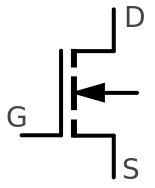
\includegraphics[width=0.05\textwidth]{pics/nFET}} & positiv & positiv \\
		\hline
		p-FET & \raisebox{-.8\totalheight} {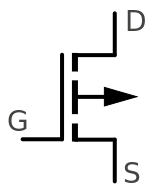
\includegraphics[width=0.05\textwidth]{pics/pFET}} & negativ & negativ \\
		\hline
	\end{tabular}
$$\hspace{-1.5cm}\text{Gatteräquivalent } n_{ge} = \frac{n_{trans}}{4}$$\\

\subsection{Zahlensysteme}
\subsubsection{Binär}
\paragraph{Bereichsüberschreitung Zweierkomplement}
\begin{itemize}
	\item [] Richtig $\Rightarrow Carry_n = Carry_{n-1}$\\
		  Falsch $\Rightarrow Carry_n \neq Carry_{n-1}$\\
\end{itemize}

\paragraph{Umwandeln von Komastellen}
\begin{itemize}
	\item [] $Komastelle_0 \cdot Basis = Ganzzahl_1,Komastelle_1$\\
		     $\dots$Weiterführen bis Genauigkeit erreicht ist\\		     
                     $Komastelle_{n-1} \cdot Basis = Ganzzahl_{n}, Komastelle_{n}$\\
			
	\item [] Wert hinter Koma in neuem Zahlensystem $= Ganzzahl_{1}\cdot Basis^{-1} + \dots+ Ganzzahl_n\cdot Basis^{-n}$\\
		Somit werden Stellen hinter Komma von oben nach unten aufgeschrieben

	\item [] \textbf{Beispiel} mit Zahl 2.7$_{10}$\\
		$\left.\begin{array}{ccc}
			2 / 2 & = 1 & R 0\\
			1 / 2 & = 0 & R 1
		\end{array}\right\uparrow$\\
		$\left.\begin{array}{cccl}
			0.7 \cdot 2 &= &\mathbf{1}.4\\
			0.4 \cdot 2 &= &\mathbf{0}.8\\
			0.8 \cdot 2 &= & \mathbf{1}.6\\
			0.6 \cdot 2 &= & \mathbf{1}.2\\
		\end{array}\right\downarrow$\\
		
		Zahl = 10,\textbf{1011}$\dots_2$ \\
	\end{itemize}
\end{multicols}
\vspace{-20pt}

	%\newpage
	%\section{Allgm. Wissen}
\subsection{Analog}
	\begin{compactitem}
		\item Die reale Welt ist analog (z.B. Sinnesorgane)
		\item Die analoge Verarbeitung stellt das Ergebnis einer Berechnung praktisch sofort zur Verfügung.
		\item Analoge Systeme sind anfällig auf externe Störsignale.
		\item Analoge Systeme sind extrem aufwändig und erfordern viel Fachwissen.	
	\end{compactitem}
	
\subsection{Digital}
	\begin{compactitem}
		\item Einfacher automatisierbarer Entwurf und Test mit Hilfe von CAD möglich.
		\item Digitale Schaltungen werden als integrierte Schaltungen mit Transistoren hergestellt uns sind somit reproduzierbar.
		\item Digitale Systeme sind bis zu einem gewissen Grad weitgehend immun gegen Störsignale.
	\end{compactitem}
	
\subsection{Unterschied Analog zu Digital}
\begin{multicols}{3}
	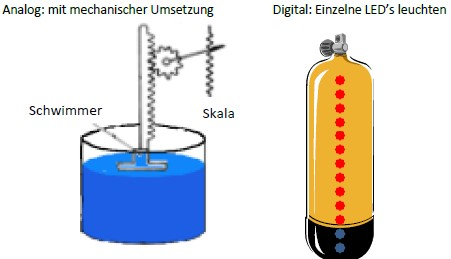
\includegraphics[width=5cm]{pics/unterschied_analog_digital.jpg}
		\columnbreak
	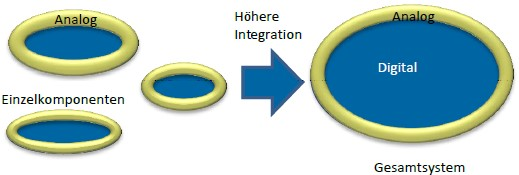
\includegraphics[width=5cm]{pics/analog_digital_integration.jpg}
		\columnbreak
		\\
	Trend zu höherer Integration: Der digitale Anteil wächst, wobei der analoge Teil weiterhin die Verbindung nach Aussen darstellt \lbrack wie eine Schale\rbrack.
\end{multicols}

	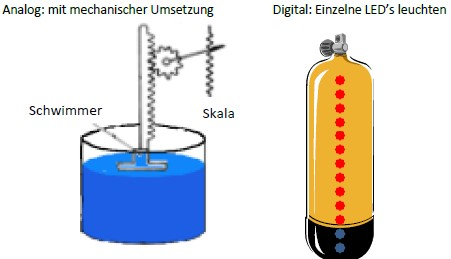
\includegraphics[width=0.3\textwidth]{pics/unterschied_analog_digital.jpg}
	
	\subsubsection{Integration}
		\begin{minipage}[c]{8 cm}
			\includegraphics[width=0.9\textwidth]{pics/analog_digital_integration.jpg}
		\end{minipage}
		\begin{minipage}[c]{10 cm}
			Trend zu höherer Integration: Der digitale Anteil wächst, wobei der analoge Teil weiterhin die Verbindung nach Aussen darstellt \lbrack wie eine Schale\rbrack.
		\end{minipage}
	
\subsection{Codes}
	\begin{minipage}[c]{5 cm}
		\includegraphics[width=0.9\textwidth]{pics/codes.jpg}
	\end{minipage}
	\begin{minipage}[c]{13 cm}
		Folgende Codes werden am häufigsten gebraucht:
		\begin{compactitem}
			\item Binärcode
			\item 
				\begin{tabbing}
					xxxxxxxxxxxxxxx\=xxxxxxxxxxxxxxxxxxxxxxxxxxxxxxxx\kill	
					Reiner Dualcode: \> Zuordnung von Dezimalzahlen den Bitfolgen des Dualsystems
				\end{tabbing}
			\item 
				\begin{tabbing}
					xxxxxxxxxxxxxxx\=xxxxxxxxxxxxxxxxxxxxxxxxxxxxxxxx\kill
					BCD Code: \> 
								\begin{tabular}{|lllllll|}
									\hline
										Dezimal & 1 & 2 & 3 & $\dots$ & 9 & \textgreater 9 \\
										BCD & 0001 & 0010 & 0011 & $\dots$ & 1001 & ungültig\\
									\hline
								\end{tabular}
				\end{tabbing}
		\end{compactitem}
	\end{minipage}

\subsection{Begriffe im Zusammenhang mit dem binären Zahlensystem}
	\begin{compactitem}	
		\item 
			\begin{tabbing}
				xxxxxxxxxxx\=xxxxxxxxxxxxxxxxxxxxxxxxxxxxxxxxxxxxx\kill	
				Bit (b): \>
							Binary Digit: Kleinsmögliche Speichereinheit in der Digitaltechnik. Kann zwei mögliche Zustände\\
				 		\>	annehmen: 0 und 1
			\end{tabbing}
		\item 
			\begin{tabbing}
				xxxxxxxxxxx\=xxxxxxxxxxxxxxxxxxxxxxxxxxxxxxxxxxxxx\kill	
				Byte (B): \>
							Einheit von 8 Bits. Auch genannt Oktett: 1 Oktett = 1 Byte = 8 Bit. Byte ist die Standartbezeichnung\\
						\>	von Speicherkapazitäten und Datenmengen.
			\end{tabbing}
		\item 
			\begin{tabbing}
				xxxxxxxxxxx\=xxxxxxxxxxxxxxxxxxxxxxxxxxxxxxxxxxxxx\kill	
				Nibble: \>
							Binärzahlen in Gruppen von 4 Bits
			\end{tabbing}
		\item 
			\begin{tabbing}
				xxxxxxxxxxx\=xxxxxxxxxxxxxxxxxxxxxxxxxxxxxxxxxxxxx\kill	
				MSB: \>
							Most Significant Bit. Bit mit höchster Wertigkeit, steht ganz links im binären Wort
			\end{tabbing}
		\item 
			\begin{tabbing}
				xxxxxxxxxxx\=xxxxxxxxxxxxxxxxxxxxxxxxxxxxxxxxxxxxx\kill	
				LSB: \>
							Least Significant Bit. Bit mit tiefster Wertigkeit, steht ganz rechts im binären Wort
			\end{tabbing}
	\end{compactitem}

	\begin{minipage}{8 cm}
	Weil sequentielle Schaltungen in der Regel synchron arbeiten, muss eine Referenz zur Einhaltung der Synchronit"at definiert werden. Das Taktsignal ist ein bin"ares Signal, das in regelm"assiger Abfolge zwischen zwei Zust"anden hin und her pendelt.
	\end{minipage}a

	\subsubsection{Unterschied Flipflop und Latch}
		\begin{minipage}{12 cm}
			Taktzustandsgesteuerte Systeme haben den Nachteil, dass in ihrer transparenten Phase auch asynchrone Schaltvorg"ange stattfinden k"onnen. Echt synchrone Systeme "andern ihren Zustand nur bei der aktiven Flanke des Taktsignals. Genau in diesem Moment und sonst nie wird das Eingangssignal bei einem Speicherelement in den Speicher "ubertragen. Nur beim taktflankengesteuerten System wechseln die Ausg"ange immer genau zum Zeitpunkt der aktiven Taktflanke. Beim taktzustandsgesteuerten System sind w"ahrend der transparenten Phase auch Zustands"anderungen zwischen zwei Taktflanken m"oglich. \\
			Taktflankengesteuerte Speicherelemente werden Flip-Flops genannt. Taktzustandsgesteuerte Speicherelemente werden Latches genannt
		\end{minipage}
		\begin{minipage}{0.5 cm}
			\ 
		\end{minipage}
		\begin{minipage}{6 cm}
			\includegraphics[width=0.9\textwidth]{pics/flipflop_latch}
		\end{minipage} 	%include -> neue Seite; f�r Formelsammlung Pr�fung auskommentieren
\end{document}

